\chapter{Laboratorio 2: \\FSM State Assignment and VHDL Synthesis}
\section{FSM State Assignment}
Durante la prima parte dell'esercitazione di laboratorio, viene richiesto di implementare un circuito per sommare 6 numeri
\begin{center}
	$s=a+b+c+d+e+f $
\end{center}
utilizzando un unico sommatore, due multiplexer e un registro.
Il circuito completo è riportato in Figura \ref{circuito}, mentre la FSM è presente in Appendice, Figura \ref{fsm}. \\
\begin{figure}[!htb]
	\centering
	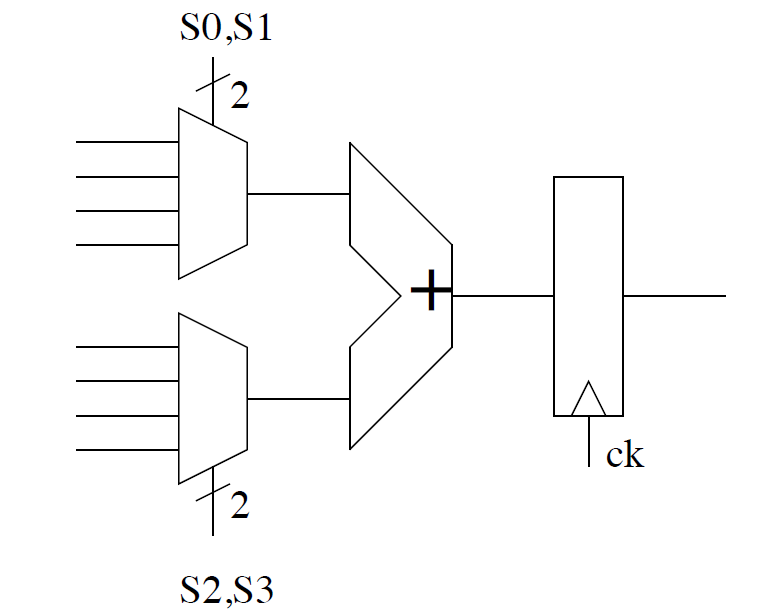
\includegraphics[scale=0.6]{immagini/circuito}
	\caption{\textit{Datapath}}
	\label{circuito}
\end{figure}
\\
Viene richiesto di valutare e minimizzare il consumo di potenza, andando a modificare la connessione degli input A-H considerando esclusivamente l'attività della FSM e i bit di selezione del MUX S0-S3.\\
Dopo varie ottimizzazioni, si è arrivati ad avere un'attività totale pari a 8 per il multiplexer e a 6 per la State transition della macchina a stati, andando a considerare che la macchina a stati e il multiplexer ricomincino le operazioni una volta terminate. Nella tabella \ref{tab2} viene riportata la configurazione degli stati e dei bit del multiplexer scelta:
\begin{table}[!h]\footnotesize
	\centering
	\begin{tabular}{|c|c|}
		\hline
		\textbf{STATI} & \textbf{$S_{3}S_{2}S_{1}S_{0}$}\\
		\hline
		000 & 0000\\
		\hline
		001 &0101 \\
		\hline
		011& 0111\\
		\hline
		010& 1110\\
		\hline
		110& 1010\\
		\hline 
	\end{tabular}
	\caption{\textit{Tabella degli stati}}
	\label{tab2}
\end{table} \\
\section{VHDL synthesis}
Il secondo punto del laboratorio prevede di sintetizzare l’FSM tramite \textit{Synopsys} e studiarne le caratteristiche in termini di area, potenza e timing in modo da ricercare possibili ottimizzazioni. Si è utilizzata la libreria a 45 nm, definito un segnale di clock di periodo corrispondente a 10 ns e si è verificato il corretto inserimento tramite il comando \emph{$report\_clock$}. In seguito si è sintetizzato il circuito
\begin{table}[!h]\footnotesize
	\centering
	\begin{tabular}{|c|c|c|}
		\hline
		\textbf{clock} & \textbf{period} & \textbf{waveform}\\
		\hline
		CLK & 10.00 ns & \{0 5\} V\\
		\hline
	\end{tabular}
	\caption{\textit{Report clock}}
\label{clock_report}
\end{table} \\
Di seguito è riportato lo schema generato da Synopsys:\\
\newpage
\begin{figure}[!htb]
	\centering
	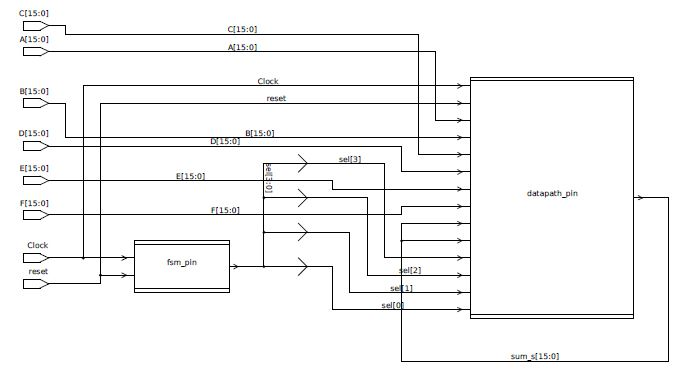
\includegraphics[scale=0.6]{immagini/schemlab2_2}
	\caption{\textit{Schematico del circuito sintetizzato}}
	\label{datapath}
\end{figure} 
\noindent Si è poi andato ad analizzare il report relativo all'area, dove si sono ottenuti informazioni riguardanti la quantità di componenti e connessioni, raccolte in Tabella \ref{numcomp} e riguardanti l'area occupata dalla logica, raccolte in Tabella \ref{areatype}. Si può ben notare come l'area relativa alla logica combinatoria sia circa il doppio di quella della logica non combinatoria e che dunque pesi per circa $\frac{2}{3}$ sull'area totale.
\begin{table}[!h]\footnotesize
	\centering
	\begin{tabular}{|c|c|}
		\hline
		\textbf{type} & \textbf{number}\\
		\hline
		ports & 114\\
		\hline
		nets & 118\\
		\hline
		cells & 2\\
		\hline
		references & 2\\
		\hline
	\end{tabular}
	\caption{\textit{Numero componenti per tipologia}}
\label{numcomp}
\end{table} \\
\begin{table}[!h]\footnotesize
	\centering
	\begin{tabular}{|c|c|}
		\hline
		\textbf{area type} & \textbf{value}\\
		\hline
		combinational & 195.244003\\
		\hline
		noncombinational & 101.08003\\
		\hline
		total cell & 296.324006\\
		\hline
	\end{tabular}
	\caption{\textit{Area occupata dalla logica}}
\label{areatype}
\end{table} \\
Successivamente, dopo aver verificato la correttezza della codifica degli stati della FSM, si è analizzato il timing del circuito, dal quale si sono ottenute importanti informazioni riguardo ai ritardi delle varie porte e soprattutto riguardo lo \textit{Slack Time}, parametro che consente di ottimizzare frequenza di funzionamento del circuito. Nel caso preso in considerazione lo Slack Time peggiore risulta pari a 8.03 ns. Ciò si evince analizzando il timing per i 10 peggiori percorsi critici e raccogliendo informazioni sullo Slack Time che sono sintetizzate nella Tabella \ref{slack1}
\begin{table}[!h]\footnotesize
	\centering
	\begin{tabular}{|c|c|}
		\hline
		\textbf{Slack (MET)} & \textbf{value [ns]}\\
		\hline
		1 & 8.04\\
		\hline
		2 & 8.04\\
		\hline
		3 & 8.04\\
		\hline
		4 & 8.04\\
		\hline
		5 & 8.04\\
		\hline
		6 & 8.05\\
		\hline
		7 & 8.05\\
		\hline
		8 & 8.05\\
		\hline
		9 & 8.05\\
		\hline
		10 & 8.05\\
		\hline
	\end{tabular}
	\caption{\textit{I dieci percorsi con timing peggiore}}
\label{slack1}
\end{table} \\
Non si evidenziano rilevanti differenze tra i diversi Slack, ciò è sicuramente dovuto alla simmetria dei percorsi critici che presentano la stessa struttura. 
Nel grafico in Figura \ref{slackgrafico} si può notare la distribuzione dei peggiori Slack:
\begin{figure}[!htb]
	\centering
	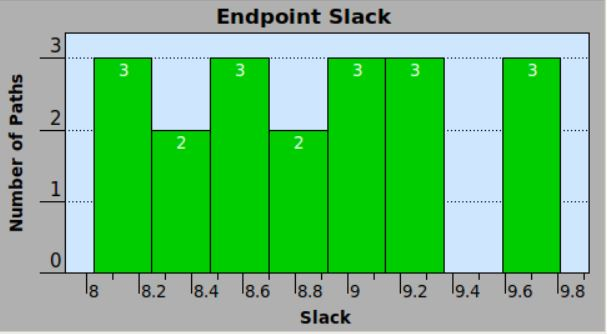
\includegraphics[scale=0.6]{immagini/slacks}
	\caption{\textit{Grafico distribuzione slacks}}
	\label{slackgrafico}
\end{figure} \\
Dunque si è analizzata la potenza dissipata sia dall’intera logica sia da ogni singola cella.
Il report sulla potenza distingue la potenza dissipata \textit{dinamicamente}, \textit{staticamente} e quella dovuta alle \textit{correnti di leakage}, fornendo la percentuale rispetto alla potenza dissipata totale e analizzando il circuito a livello gerarchico. Il report è sintetizzato nella Tabella \ref{pot}. In questo modo è possibile capire quanto influiscono i diversi contributi di potenza e nel caso intervenire in modo specifico per ridurre opportunamente i consumi.
\begin{table}[!h]\footnotesize
	\centering
	\begin{tabular}{|c|c|c|c|c|c|}
		\hline
		\textbf{hierarchy} & \textbf{switch} & \textbf{int} & \textbf{leak}& \textbf{tot}& \textbf{\%}\\
		\hline
		m\_adder & 11.943 & 28.443 & 5.46e+3 & 45.844 & 100\\
		\hline
		datapath\_adder & 10.930 & 25.532 & 5.03e+3 & 41.495 & 90.5\\
		\hline
		add\_78 & 1.765 & 4.921  & 1.19e+3 & 7.879 & 17.2\\
		\hline
		fsm & 1.012 & 2.911 & 425.171 & 4.349 & 9.5\\
		\hline
	\end{tabular}
	\caption{\textit{Consumi dei vari blocchi}}
\label{pot}
\end{table} \\
Inoltre si è  analizzata l’attività delle singole celle in modo da studiare i consumi di ogni singola cella  e se ne riporta il report in Tabella \ref{cellpot}. Da quest'ultimo si può notare come la cella che consuma di più, sia a livello di leakage che a livello di potenza dinamica sia il \textit{Register}.
\begin{table}[!h]\footnotesize
	\centering
	\begin{tabular}{|c|c|c|c|c|}
		\hline
		\textbf{cell} & \textbf{cell internal} & \textbf{driven net switching} & \textbf{tot dynamic [\% cell/tot]}& \textbf{cell leakage}\\
		\hline
		REG[0] & 1.0163 & 0.0584 & 1.075 (95\%) & 87.1072\\
		\hline
		REG[1] & 0.8660 & 0.1134 & 0.979 (88\%) & 81.4649\\
		\hline
		REG[2] & 0.7468 & 0.1083 & 0.855 (87\%) & 84.7325\\
		\hline
		U8 & 0.0465 & 0.0297 & 7.62e-2 (61\%) & 33.6813\\
		\hline
		U9 & 0.0386 & 0.1368 & 0.175 (22\%) & 31.6341\\
		\hline
		U6 & 0.0375 & 0.1356 & 0.173 (22\%) & 18.0848\\
		\hline
		U5 & 0.0314 & 0.0193 & 5.07e-2 (62\%) & 19.3118\\
		\hline
		U4 & 0.0304 & 0.0174 & 4.77e-2 (64\%) & 17.9767\\
		\hline
		U10 & 0.0285 & 0.0746 & 0.103 (28\%) & 12.9020\\
		\hline
		U7 & 0.0233 & 0.1282 & 0.151 (15\%) & 15.8344\\
		\hline
		U3 & 0.0190 & 0.1236 & 0.143 (13\%) & 17.0242\\
		\hline
		U11 & 9.993e-3 & 0.0392 & 4.92e-2 (20\%) & 14.3532\\
		\hline
		\hline
		tot (12 cells) & 2.894 uW & 984.349 nW & 3.878 uW (75\%) & 434.107 nW\\
		\hline 
	\end{tabular}
	\caption{\textit{Attività delle singole celle}}
\label{cellpot}
\end{table} \\
Si può anche valutare il numero di commutazioni delle singole uscite valutando sia la capacità del carico che il tasso di commutazioni, raccolto il tutto in Figura \ref{attload}. In accordo con i risultati precedenti si denota un'attività più intensa per i registri in quanto risultano avere un carico capacitivo molto più alto delle altre uscite.
\newpage 
\begin{table}[!h]\footnotesize
	\centering
	\begin{tabular}{|c|c|c|c|c|}
		\hline
		\textbf{net} & \textbf{total net load} & \textbf{static prob.} & \textbf{toggle rate}& \textbf{switching power}\\
		\hline
		S[2] & 11.104 & 0.326 & 0.0244 & 0.1641\\
		\hline
		S[0] & 9.304 & 0.228 & 0.0244 & 0.1375\\
		\hline
		S[1] & 10.166 & 0.295 & 0.0221 & 0.1360\\
		\hline
		S[3] & 9.541 & 0.186 & 0.0200 & 0.1153\\
		\hline
		n21 & 10.518 & 0.088 & 0.0181 & 0.1153\\
		\hline
		n5 & 6.169 & 0.814 & 0.0200 & 0.0746\\
		\hline
		n6 & 3.949 & 0.772 & 0.0244 & 0.0584\\
		\hline
		n8 & 4.078 & 0.706 & 0.0222 & 0.0546\\
		\hline
		n25 & 3.843 & 0.500 & 0.0221 & 0.0514\\
		\hline
		n28 & 6.482 & 0.772 & 0.0100 & 0.0392\\
		\hline
		n27 & 1.980 & 0.706 & 0.0244 & 0.0293\\
		\hline
		N8 & 1.438 & 0.098 & 0.0221 & 0.0193\\
		\hline
		n7 & 1.438 & 0.0392 & 0.0200 & 0.0174\\
		\hline
		\hline
		tot (13 nets) &  &  &  & 1.0125 uW\\
		\hline 
	\end{tabular}
	\caption{\textit{Carico, toggle rate e consumo dei vari nodi}}
\label{attload}
\end{table}
\noindent Adesso si focalizza l’attenzione sui consumi della Macchina a Stati. La FSM è caratterizzata da una Potenza dovuta alla \textit{Corrente di Leakage} di 418 nW a fronte dei 434 nW totali, ma si può notare come anche per gli altri contributi di potenza i dati tendono ad evidenziare il ruolo preponderante della macchina a stati sui consumi complessivi. Il tutto è raccolto in Figura \ref{fsm_power_cell}.\\
\begin{figure}[!htb]
	\centering
	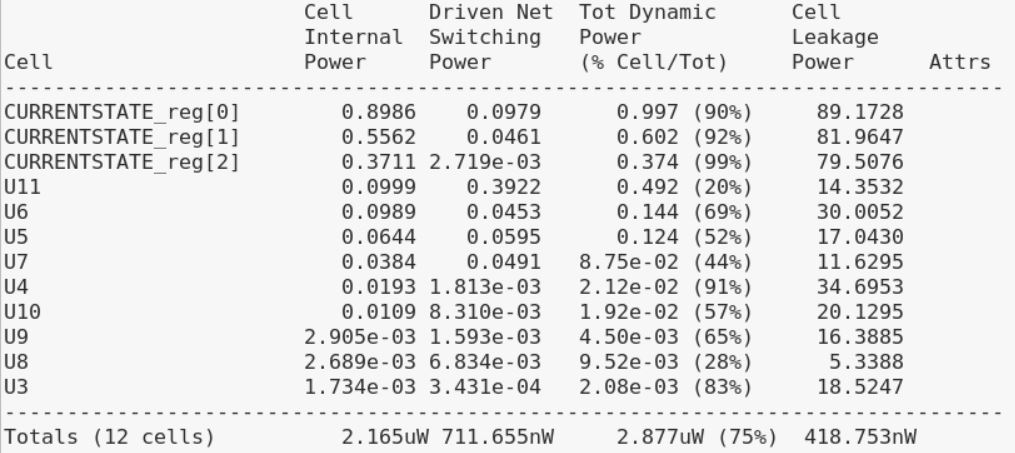
\includegraphics[scale=0.6]{immagini/fsm_power_cell}
	\caption{\textit{Potenza dissipata dalla FSM}}
	\label{fsm_power_cell}
\end{figure}
Dopodiché si è provato a variare la frequenza di lavoro del circuito, provando a sintetizzare il circuito in modo da lavorare alla massima frequenza di funzionamento consentita dal percorso critico. Dall’analisi sul timing si era trovato che lo Slack Time peggiore era di circa 8.02 ns lavorando con un periodo di clock pari a 10 ns. Di conseguenza si deduce che si può decrementare il periodo di clock fino a $10 ns-8.02 ns=1.98 ns$. Si è scelto così un periodo di Clock pari a 2 ns.
\\
\begin{table}[!h]\footnotesize
	\centering
	\begin{tabular}{|c|c|}
		\hline
		cell internal power & 141.4894 uW (71\%)\\
		\hline
		net switching power & 58.8064 uW (29\%)\\
		\hline
		\hline
		total dynamic power & 200.2958 uW (100\%)\\
		\hline
		cell leakage power & 5.5273 uW\\
		\hline
	\end{tabular}
	\caption{\textit{Tabella consumi}}
\label{conslack}
\end{table} \\
Dalla Tabella \ref{conslack} si nota come sia aumentata la Total Dynamic Power, in quanto aumentando la frequenza operativa aumentano anche il numero di commutazioni interne e quindi viene dissipata maggiore potenza dinamica. Resta invece invariata la corrente di leakage che infatti dipende solo dalla tecnologia usata.\\
Infine è stato posto al sintetizzatore un ulteriore vincolo sulla massima potenza dinamica dissipabile, fissandola a $200 \mu W$, considerando che nell’ultimo report la potenza totale dissipata ammonta a $200.2958 \mu W$. Viene riportato il report in Tabella \ref{potadesso}\\
\begin{table}[!h]\footnotesize
	\centering
	\begin{tabular}{|c|c|}
		\hline
		cell internal power & 140.3547 uW (70\%)\\
		\hline
		net switching power & 59.0397 uW (30\%)\\
		\hline
		\hline
		total dynamic power & 199.3944 uW (100\%)\\
		\hline
		cell leakage power & 5.5832 uW\\
		\hline
	\end{tabular}
	\caption{\textit{Tabella consumi}}
\label{potadesso}
\end{table}
\\
Adesso la potenza dinamica totale dissipata è di $199.3944 \mu W$ e rispetta il vincolo.
Inoltre, si nota che stavolta il parametro della potenza di leakage è leggermente variato, poichè stavolta per rispettare il vincolo sul consumo di potenza è stata variata la topologia del circuito usando differenti porte logiche.

